\section*{Lecture 1: Sets and Maps (Sep. $3^{rd}$)}

% SETS
\subsection*{\colorbox{yellow}{Sets.}}
\qquad A set is a collection of distinct elements. If an element \(x\) is in the set \(S\), we write \(x \in S\). If \(x\) is not, then we write \(x \notin S\).\\ 
\, \\
\textbf{Example:} $\mathbb{P} = \{ x \mid x \text{ is a prime number} \}$. From the set definition, we know that: \(5 \in \mathbb{P},\, 4 \notin \mathbb{P}\).\\

\begin{enumerate}
    \item \textbf{Some useful sets:} 
    \[
        \mathbb{R}: \text{ Reals},\quad \mathbb{Q}: \text{ Rationals},\quad \mathbb{Z}: \text{ Integers},\quad \mathbb{N}: \text{ Naturals}.
    \]
    \item \textbf{Describing a set:}
        \begin{itemize}
            \item Listing all of the elements in the set (Remark: Ordering in a set does not matter):
            \begin{itemize}
                \item \(A = \{1, 2, 3\} \qquad B = \{2, 0, -1\}\) 
            \end{itemize}
            \item Specifying the characteristics/properties:
            \begin{itemize}
                \item \(C = \{ n \in \mathbb{N} :\, 4 \mid n \}\)
            \end{itemize}
            \item The set with no elements is called the empty set, and it is \textbf{denoted as \(\varnothing\) instead of \{\}}.
        \end{itemize}
    \item \textbf{Subset:} If \(S, T\) are sets such that all elements of \(S\) are contained in \(T\), we say that \(S\) is a subset of \(T\) (we write \(S \subset T\)).
    \item \textbf{Sets equality:} Two sets contain exactly the same elements; we write \(S = T\). 
        \[ S = T \Leftrightarrow (S \subset T) \land (T \subset S)\]
    \item \textbf{Proper Subset:} If \(S \subset T\) but \(T \neq S\), then we say \(S\) is a proper subset of \(T\) and we write \(S \subsetneq T\).
        \[A \subsetneq B \Leftrightarrow \forall x \, (x \in A \implies x \in B) \land \exists x \, (x \notin A \land x \in B)\]
    \item \textbf{Operations on sets:} 
        \begin{itemize}
            \item \textbf{Union (\(\cup\)):} If \(S, T\) are sets, the union of \(S\) and \(T\) is:
                \[S \cup T = \{x \mid (x \in S) \lor (x \in T)\}\]
            \item \textbf{Intersection (\(\cap\)):} If \(S, T\) are sets, the intersection of \(S\) and \(T\) is:
                \[S \cap T = \{x \mid (x \in S) \land (x \in T)\}\]
            \item \textbf{Example:} Let \(\mathbf{N} = \{x \in \mathbb{Z} \mid x > 0\} = \{1, 2, 3, 4, \dots\}\) be the set of natural numbers, and let \(-\mathbf{N} = \{x \in \mathbb{Z} \mid x < 0\}\) be the set of negative integers. We can have the following operations:
                \[\mathbf{N} \cup -\mathbf{N} = \{x \in \mathbb{Z} \mid x \neq 0\}\]
                \[\mathbf{N} \cap -\mathbf{N} = \varnothing \quad \text{(Disjoint)}\] 
            \item \textbf{Union and Intersection over multiple sets:} If we have a list of sets \(S_1, S_2, \dots, S_k\), we can form their union and intersection using the following representations:
                \[\textbf{Union of all sets:}\quad\bigcup_{i=1}^{k} S_i = \{x \mid x \in S_i, \, \exists S_i, i = 1, \dots, k\}\]
                \[\textbf{Intersection of all sets:}\quad\bigcap_{i=1}^{k} S_i = \{x \mid x \in S_i, \, \forall i = 1, \dots, k\}\]
        \end{itemize}
\newpage
    \item \textbf{Relations on Sets:} A relation on a set \(A\) is a rule for determining whether, for any elements \(x\) and \(y\) in \(A\), \(x\) stands in a given relationship to \(y\).
        \begin{itemize}
            \item \textbf{Relation:} A relation on \(A\) is any set \(S\) of ordered pairs of elements of \(A\). The elements \(x\) and \(y\) satisfy the relation \textbf{iff} \((x, y) \in S\).
                \begin{itemize}
                    \item Example: \quad \(\forall x \in \mathbb{R}, \exists y \in \mathbb{R}, x \leq y\) \quad (The "greater than or equal to" relation in reals)
                \end{itemize}
            \item \textbf{Equivalence Relations:} A special type of relation, \(S\) is an \textbf{equivalence relation} on \(A\) if it satisfies:
                \begin{enumerate}
                    \item \textbf{Reflexivity:} \(\forall x \in A, \, x \sim x\)
                    \item \textbf{Symmetry:} \(x \sim y \implies y \sim x\)
                    \item \textbf{Transitivity:} \((x \sim y) \land (y \sim z) \implies x \sim z\)
                \end{enumerate}
                
                \subsubsection*{Example:}
                Has the same birthday relation: Consider a set \(A\) of people. Define a relation \(R\) on \(A\) such that for any two people \(a, b \in A\):
                \[
                a \, R \, b \text{ if and only if } a \text{ and } b \text{ have the same birthday}.
                \]
                \begin{itemize}
                    \item \textbf{Reflexive:} Every person has the same birthday as themselves, so \(a \, R \, a\) for all \(a \in A\).
                    \item \textbf{Symmetric:} If \(a \, R \, b\), then \(b \, R \, a\), since having the same birthday works both ways.
                    \item \textbf{Transitive:} If \(a \, R \, b\) and \(b \, R \, c\), then \(a \, R \, c\), since if \(a\) shares a birthday with \(b\) and \(b\) with \(c\), then \(a\) and \(c\) share the same birthday.
                \end{itemize}
                This ``has the same birthday" relation is an equivalence relation. The equivalence classes are groups of people who share the same birthday.

                \subsubsection*{Question:} 
                \qquad Provide an example of an equivalence relation.
        \end{itemize}
\end{enumerate}

\vspace*{- 0.1cm}


% FUNCTIONS
\subsection*{\colorbox{yellow}{Functions.}}
\qquad If S and T are sets, then a \textbf{function} $f$ from S to T, denoted \(f: \, S \rightarrow T\), is a rule assigning to each $x \in S$ an unique element $f(x)\in T$. 
    \begin{enumerate}
        %
        \item \textbf{Terminologies:}
            \begin{itemize}
                \item $f(x)$ is the \textbf{image of $x$ under $f$}.
                \item \(\forall x \in S \), \( x \) is called the \textbf{preimage of } \( f(x) \) \textbf{ under } \( f \).
                \item S is the \textbf{domain} of $f$, $T$ is the \textbf{codomain} of $f$, the \textbf{range of $f$} is the set:
                    \(\{f(x) \mid x \in S\} \subset T\)
                \item \textbf{Codomain:} of a function  $f: S \rightarrow T$  is the set  $T$  that includes all potential values the function could map to. It is specified when defining the function, but not every element in the codomain is necessarily an output of the function.
                \end{itemize}
        %
        \item \textbf{Image and Preimage of Subsets under a Function:}
                \begin{itemize}
                    \item If $U \subset S$ is a subset, then the image of $U$ is:
                        \[ f(U) = \{f(x) \mid x \in U\}\]
                    \item If $V \subset T$, then the preimage of $V$ is:
                        \[ f^{-1}(V) = \{x \mid f(x) \in V\}\]
                    \item If \( f: S \rightarrow T \) and \( U \subseteq S \), then the restriction of \( f \) to \( U \), denoted \( f|_U \), is defined by
                        \[ f|_U(x) = f(x) \quad \text{for all } x \in U. \]
                \end{itemize}
            \vspace{-0.8cm}
            \subsubsection*{Example.}
            \qquad Let $S = \{x \in \mathbb{R} \mid \, |x| \ge 1\}$ and let $f: S \rightarrow \mathbb{R}$ be the function sends $x$ to \(\frac{1}{x^{2}}\),
                \[f(x) = \frac{1}{x^{2}}\]
            \vspace*{-0.2cm}
            \begin{itemize}
                \item The domain is S, the codomain is $\mathbb{R}$, and the range is \((0,1]\).
                \item Since \( f(2) = \frac{1}{4} \), then \( \frac{1}{4} \) is the image of 2. \(-2\) is also the preimage of \( \frac{1}{4} \).
                \item The image of \([1, 10]\) is \(\left[ \frac{1}{100}, 1 \right]\) and the preimage of \((0, \frac{1}{2})\) is \((\sqrt{2}, \infty) \cup (-\infty, -\sqrt{2})\).
            \end{itemize}
            \vspace*{0.5cm}
        %
        \item \textbf{Types of functions:}
            \begin{itemize}
                \item \textbf{Injection (One-to-one):} If every element in the range has a unique preimage, we say $f$ is injective.
                \item \textbf{Surjection (Onto):} If every element in the codomain of $f$ is in the range of $f$, we say $f$ is surjective.
                \item \textbf{Bijection (One-to-one and Onto):} If $f$ is surjective and injective, we say $f$ is bijective.\\
                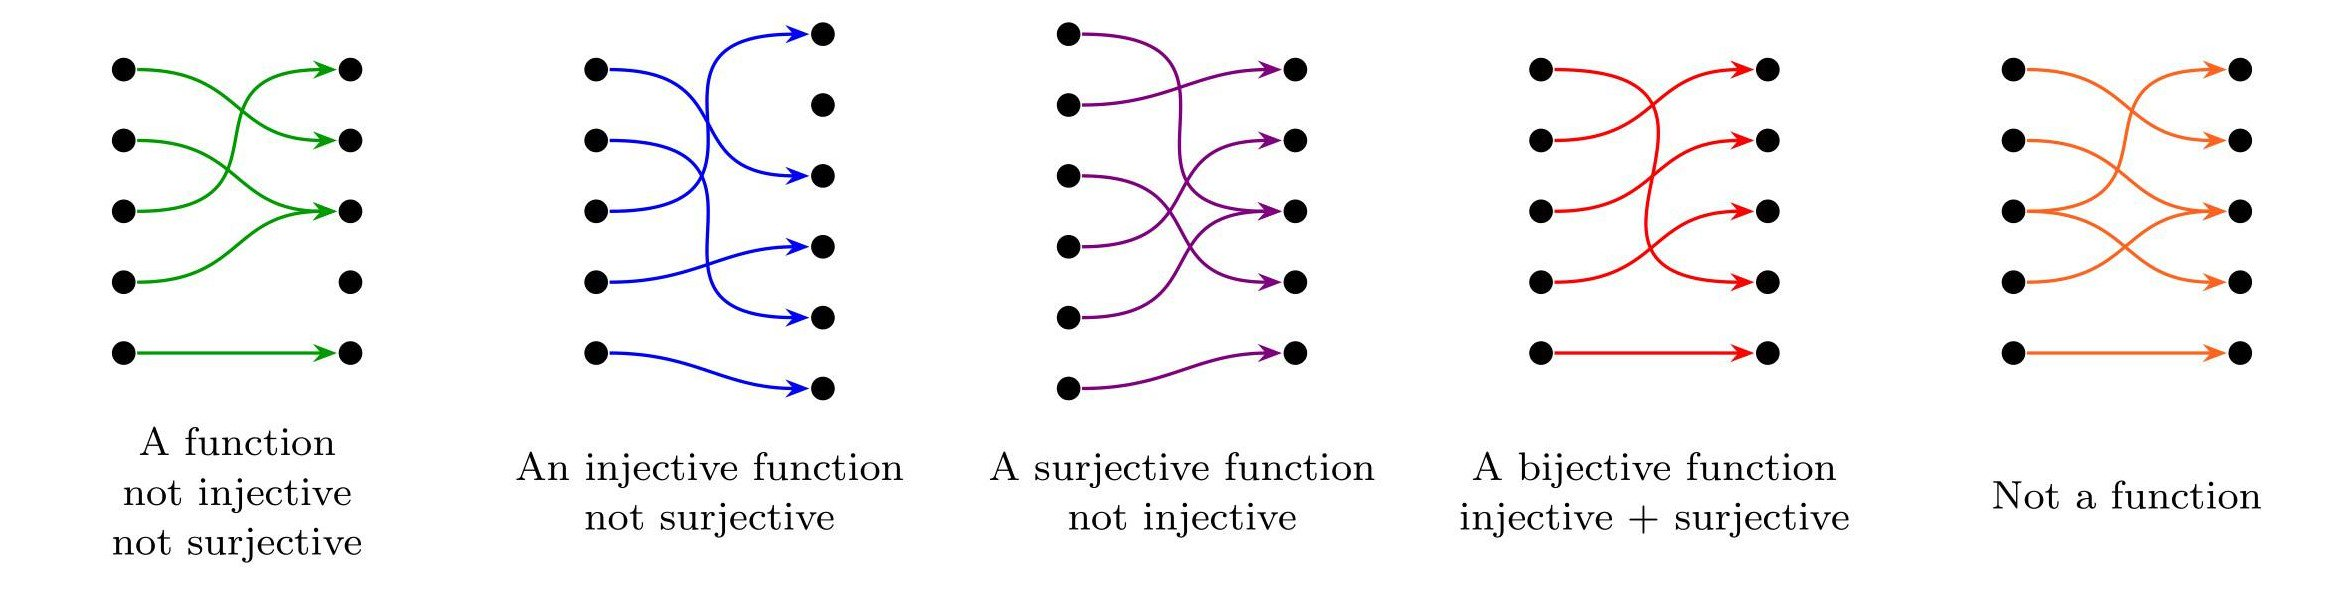
\includegraphics[width = 0.85\textwidth]{images/types-of-functions.jpeg}
            \end{itemize}
                \subsubsection*{Example.}
                    Let \( f: \mathbb{Z} \rightarrow \mathbb{N} \) be defined by \( f(x) = |x| + 1 \). Then \( f \) is surjective but not injective. The function \( f|_{\mathbb{N}} \) is injective but not surjective. Let \( \mathbb{Z}_{\geq 0} = \{ x \in \mathbb{Z} : x \geq 0 \} \). Then \( f|_{\mathbb{Z}_{\geq 0}} \) is both injective and surjective, hence a bijection. 
                \vspace*{0.5cm}
        %
        \item \textbf{Composition of functions:}\\ \\
            If \( f: S \rightarrow T \) and \( g: T \rightarrow U \) are functions, then the function which sends \( x \in S \) to \( g(f(x)) \) is the composite \( g \circ f: S \rightarrow U \), so \( g \circ f(x) = g(f(x)) \). \textcolor{red}{Remark: Even if \( f, g: S \rightarrow S \), we don’t necessarily have \( f \circ g = g \circ f \).} \\ \\
            \textbf{Exercise:} produce an example.\\
            \vspace*{0.5cm}
        \item \textbf{Inverse function:}\\ 
            Finally, a function \( f: S \rightarrow T \) is invertible if there exists a function \( g: T \rightarrow S \) such that
            \[
            g \circ f(x) = x \quad \forall x \in S, \quad \text{and} \quad f \circ g(y) = y \quad \forall y \in T.
            \]
            If it exists, such a \( g \) is the inverse of \( f \) and is denoted \( f^{-1} \).

            \textbf{Exercise.} Show that \( f \) is invertible iff it is bijective.

            \textbf{Example.} For the inverse of our function \( f: \mathbb{Z}_{\geq 0} \rightarrow \mathbb{N} \) from the last example is simply\\ \( f^{-1}(y) = y - 1 \).       
        \end{enumerate}
    
    

